\documentclass{article}
\usepackage[utf8]{inputenc}

\usepackage{natbib}
\usepackage{amsthm}
\usepackage{amssymb}
\usepackage{float}
\usepackage{algorithm}
%\usepackage{algorithmic}
\usepackage{listings}
\lstset{
  basicstyle=\ttfamily,
  columns=fullflexible,
  frame=single,
  breaklines=true,
  tabsize=2
  %postbreak=\mbox{\textcolor{red}{$\hookrightarrow$}\space},
}
\usepackage{algpseudocode}

\usepackage{amsmath}%
\usepackage{MnSymbol}%
\usepackage{wasysym}%
\usepackage{graphicx}
\usepackage{csquotes}
\usepackage{geometry}
\geometry{
 a4paper,
 total={170mm,257mm},
 left=25mm,
 right=25mm,
 top=20mm,
 }

\begin{document}
\begin{titlepage}
\begin{center}


{\large Master 1 MoSIG}\\[0.5cm]
\vspace*{10cm}
{\Huge \textbf{Parallel Algorithms and Programming} }\\[0.5cm]
{\large Lab 5 report} \\[3cm]

% Author and supervisor
\noindent
\begin{minipage}{0.4\textwidth}

   \centering Member:\\Son-Tung \uppercase{Do}\\Johana \uppercase{Marku}

\end{minipage}%

\vfill
% Bottom of the page
{Grenoble, April 17, 2019}
\clearpage

%\tableofcontents

\end{center}
\end{titlepage}

\section{Fox Algorithm}
We successfully implemented the Fox's algorithm with MPI.
\bigskip

Since we do not handle the data distribution in this exercises, all the processes are initialized with a value $a$ and $b$ as a block of matrix A and B. Also a variable $c$ to store the result of computation of the final matrix in the same block.

Given the number or process available N, we always create a matrix of size $n \times n$ where $n \equal \sqrt{N}$ if $N \mod 2 \equal 0$ or $ \sqrt{N-1}$ if $N \mod 2 \neq 0 $

We create a grid process, and 2 sub-communicator are for row and column. The row communicator is used for broadcasting the value of matrix A as every stage, the whole row using the same value of a certain block in that row. The column matrix is used for shifting the value of matrix B.

\bigskip
\textit{N.B: The code provided has the matrix value initialized in each block corresponded to the same rank of the process holding it for the purpose of testing, the code for random value also provided}

\section{Cannon Algorithm}
We successfully implemented the algorithm with MPI. 
\bigskip

The same setup is used from the previous exercise: Matrix value initialization, Grid size, sub-communicator. The different comes from the algorithm itself, when we have to do a pre-skewing and post-skewing stage before and after the loop run. 

\bigskip
There are optimization we did in this exercise, we created more local variables to store values of matrix A and B during the shifting. Because of that, we avoid modifying the original value of matrix A and B. Thanks to this, the post-skewing stage is unnecessary. This will save us some communication cost to restore the initial state of the matrix.

\bigskip
\textit{N.B: The optimization is done in file ex2-op.c}
\section{Data distribution}
For this exercises, we tried to utilized the vector datatype of MPI by define a typeMatCol, and type MatRow. While doing the Scatterv function, we stuck dealing with distributing the MatB while MatA is run perfectly.

The only thing, we noticed is that the blocks of value that got problem are all supposed to have the same data. We have that problem and don't know how to fix it. We did try to used both dynamic allocation and static allocation.
\section{Performance Evaluation}

We did some performance test with Fox Algorithm, Cannon Algorithm, also with a sequential code (written by ourselves)

\begin{figure}[H]
	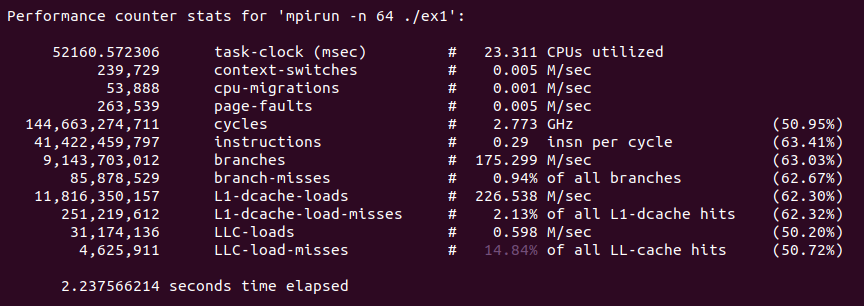
\includegraphics[width=\textwidth]{ex1.png}
	\caption{Fox algorithm with 8x8 matrix}
\end{figure}

\begin{figure}[H]
	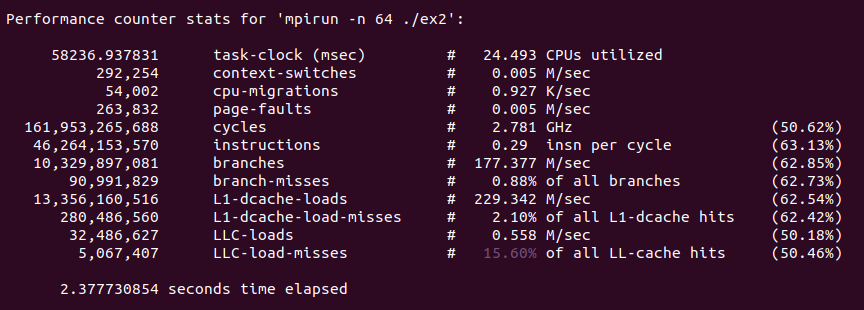
\includegraphics[width=\textwidth]{ex2.png}
	\caption{Cannon algorithm with 8x8 matrix}
\end{figure}

\begin{figure}[H]
	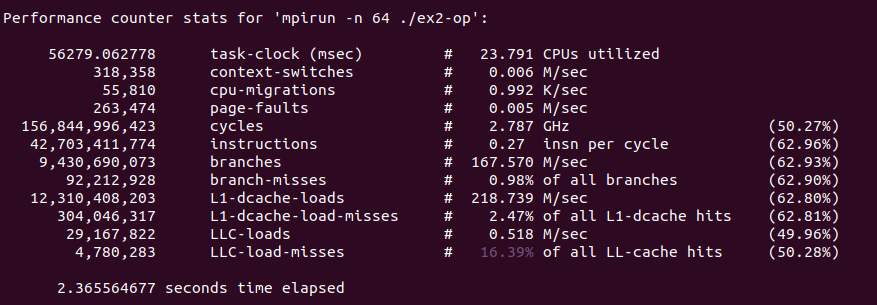
\includegraphics[width=\textwidth]{ex2-op.png}
	\caption{Cannon algorithm with 8x8 matrix (optimized version)}
\end{figure}

\begin{figure}[H]
	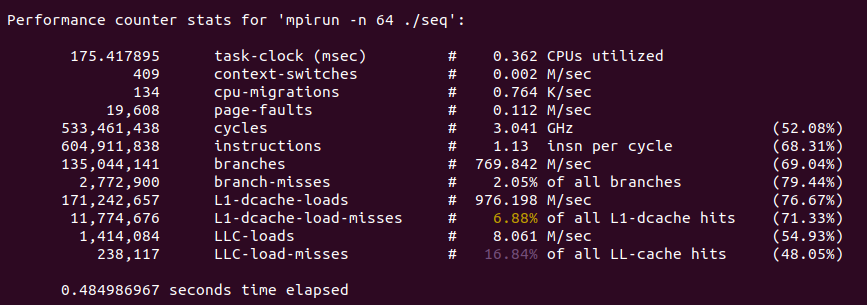
\includegraphics[width=\textwidth]{seq.png}
	\caption{Sequential with 8x8 matrix}
\end{figure}

We realized that our implementation has a very simple local computation as 1 value is hold in one process. This make the sequential time so small as they don't have communication cost.

There is one remark is our Canon optimized version actually run faster than the normal implementation. But since the size of the matrix that we test is not very big, the amount is not much.

\end{document}
